% !TEX root = summary.tex
\documentclass[8pt]{extarticle}
\usepackage[utf8]{inputenc}
\usepackage{amsmath, amsfonts, amssymb, bm}
\usepackage{graphicx, hyperref, geometry, multicol, titlesec, enumitem, color, booktabs, tikz}
\usetikzlibrary{patterns, calc, decorations.pathmorphing}

% Geometry
\geometry{a4paper, landscape, margin=0.5cm}
\setlength{\parindent}{0pt}
\setlength{\parskip}{0pt}
\setlength{\columnsep}{15pt}

% Compact lists
\setlist{nosep, leftmargin=*}
\setlist[itemize]{label=\tiny$\bullet$}

% Section formatting
\titleformat{\section}{\small\bfseries\uppercase}{}{0em}{}[\titlerule]
\titleformat{\subsection}{\footnotesize\bfseries}{}{0em}{}
\titleformat{\subsubsection}{\tiny\bfseries}{}{0em}{}
\titlespacing*{\section}{0pt}{2pt}{1pt}
\titlespacing*{\subsection}{0pt}{1pt}{0pt}
\titlespacing*{\subsubsection}{0pt}{1pt}{0pt}

\newcommand{\step}[1]{\textbf{\scriptsize Step #1:}}

\begin{document}

\begin{multicols*}{3}
\raggedcolumns
\footnotesize \textbf{STRUCTURAL MECHANICS SUMMARY PART II} \hfill \today
\vspace{2pt}
\hrule
\vspace{2pt}

\section{1. Beams}
\subsection{Theory Overview}
Beams are 1D structures ($L \gg b, h$).
\begin{itemize}[leftmargin=*]
    \item \textbf{Timoshenko}: Includes shear deformation. Valid for thick/moderately thick beams ($L/t \approx 5-10$).
    \item \textbf{Euler-Bernoulli}: Neglects shear deformation ($\gamma=0$). Valid for thin beams ($L/t > 10$). Limiting case of Timoshenko as $GA_V \to \infty$.
\end{itemize}

\subsubsection{Governing Equations}
\textbf{Timoshenko}:
\begin{align*}
    u(x,z) &= u_0(x) + z\beta(x) \\
    w(x,z) &= w(x)
\end{align*}
\textit{Constitutive}:
$N = EA u'$, $M = EI \beta'$, $V = GA_V (w'+\beta)$.
\textit{Equilibrium}:
$N' + p_x = 0$, $V' + p_z = 0$, $M' - V = 0$.

\textbf{Euler-Bernoulli}:
Constraint $\beta(x) = -\frac{w(x)}{dx}$ and $\gamma = \frac{\partial \beta}{\partial x}$.
Equation: $(EI w'')'' = p_z$.

\subsection{Problem Solving Strategy: Beams}
Use this procedure for any beam problem.

\step{1} \textbf{Identify Theory \& Geometry}
Is it thick (Timoshenko) or thin (Euler-Bernoulli)?
If unspecified, use Timoshenko for generality or Euler-Bernoulli for simplicity if explicitly allowed.
Define coordinates ($x$-axis along beam, $z$-axis downwards/transverse).

\step{2} \textbf{Integrate for Internal Forces}
Start with equilibrium equations.
\begin{itemize}
    \item Shear Force $V(x)$: Integrate load $p_z(x)$.
    \[ V(x) = -\int p_z(x) dx + C_1 \]
    \item Bending Moment $M(x)$: Integrate Shear $V(x)$.
    \[ M(x) = \int V(x) dx + C_2 = \int (-\int p_z) dx + C_1 x + C_2 \]
\end{itemize}
\textit{Tip}: If $p_z=0$, $V$ is constant ($C_1$), $M$ is linear ($C_1 x + C_2$).
\textit{Tip}: If $p_z=const$, $V$ is linear, $M$ is quadratic.

\step{3} \textbf{Integrate for Kinematics}
\textbf{Case A: Timoshenko} (3 Equations)
\begin{enumerate}
    \item Rotation $\beta(x)$: Integrate $M = EI \beta'$.
    \[ \beta(x) = \int \frac{M(x)}{EI} dx + C_3 = \frac{1}{EI} \int (C_1 x + C_2 ...) + C_3 \]
    \item Deflection $w(x)$: Integrate $V = GA_V(w'+\beta) \implies w' = \frac{V}{GA_V} - \beta$.
    \[ w(x) = \int \left( \frac{V(x)}{GA_V} - \beta(x) \right) dx + C_4 \]
\end{enumerate}
\textbf{Case B: Euler-Bernoulli} (2 Equations)
\begin{enumerate}
    \item Slope $w'(x)$: Integrate $M = -EI w''$.
    \[ w'(x) = -\int \frac{M(x)}{EI} dx + C_3 \]
    \item Deflection $w(x)$: Integrate slope.
    \[ w(x) = \int w'(x) dx + C_4 \]
\end{enumerate}

\step{4} \textbf{Apply Boundary Conditions (BCs)}
Identify support types at $x=0$ and $x=L$.
\begin{center}
\scriptsize
\renewcommand{\arraystretch}{1.5}
\begin{tabular}{@{}l c c c c c@{}}
\toprule
& 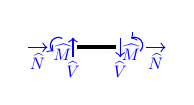
\begin{tikzpicture}[scale=0.25, baseline={(0,-0.1)}]
    \useasboundingbox (-2.5,-1.5) rectangle (4.5,1);
    \draw[line width=1.5pt] (0,0) -- (2,0);
    
    \draw[<-, blue] (-1.2, -0.2) arc (230:60:0.4) node[below, scale=0.6] {$\widehat{M}$};
    \draw[->, blue] (3.2, -0.2) arc (-50:120:0.4) node[below, scale=0.6] {$\widehat{M}$};
    
    \draw[->, blue] (-0.2,-0.5) -- (-0.2,0.5) node[below, pos=0.1, scale=0.6] {$\widehat{V}$};
    \draw[<-, blue] (2.2,-0.5) -- (2.2,0.5) node[below, pos=0.1, scale=0.6] {$\widehat{V}$};

    \draw[<-, blue] (-1.5,0) -- (-2.5,0) node[below, pos=0.5, scale=0.6] {$\widehat{N}$};
    \draw[->, blue] (3.5,0) -- (4.5,0) node[below, pos=0.5, scale=0.6] {$\widehat{N}$};
    
\end{tikzpicture} & $w$ & $\beta$ & $M$ & $V$ \\
\midrule
Clamped &
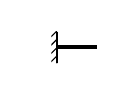
\begin{tikzpicture}[scale=0.25, baseline={(0,-0.1)}]
    \useasboundingbox (-1.5,-1.5) rectangle (2.5,1);
    \draw[line width=1.5pt] (0,0) -- (2,0);
    %\draw[decorate, decoration={snake, amplitude=0.4, segment length=4}] (2,-0.1) -- (2,0.1);
    \draw[thick] (0,-0.8) -- (0,0.8); 
    \fill[pattern=north east lines] (-0.3,-0.8) rectangle (0,0.8);
\end{tikzpicture}
& 0 & 0 & & \\

Pinned &
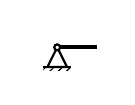
\begin{tikzpicture}[scale=0.25, baseline={(0,-0.1)}]
    \useasboundingbox (-1.5,-1.5) rectangle (2.5,1);
    \draw[line width=1.5pt] (0,0) -- (2,0);
    %\draw[decorate, decoration={snake, amplitude=0.4, segment length=4}] (2,-0.1) -- (2,0.1);
    \draw[thick] (0,0) -- (-0.5, -1) -- (0.5, -1) -- cycle;
    \draw[thick, fill=white] (0,0) circle (0.15);
    \fill[pattern=north east lines] (-0.7,-1.2) rectangle (0.7,-1);
    \draw (-0.7,-1) -- (0.7,-1);
\end{tikzpicture}
& 0 & & 0 & \\

Free end &
\begin{tikzpicture}[scale=0.25, baseline={(0,-0.1)}]
    \useasboundingbox (-1.5,-1.5) rectangle (2.5,1);
    \draw[line width=1.5pt] (0,0) -- (2,0);
    %\draw[decorate, decoration={snake, amplitude=0.4, segment length=4}] (2,-0.1) -- (2,0.1);
\end{tikzpicture}
& & & 0 & 0 \\

Tip moment &
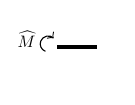
\begin{tikzpicture}[scale=0.25, baseline={(0,-0.1)}]
    \useasboundingbox (-1.5,-1.5) rectangle (2.5,1);
    \draw[line width=1.5pt] (0,0) -- (2,0);
    \draw[->] (-0.6, -0.2) arc (250:45:0.4) node[left, pos=0.5, scale=0.6] {$\widehat{M}$};
    %\draw[decorate, decoration={snake, amplitude=0.4, segment length=4}] (2,-0.1) -- (2,0.1);
\end{tikzpicture}
& & & $\widehat{M}$ & 0 \\

Tip force &
\begin{tikzpicture}[scale=0.25, baseline={(0,-0.1)}]
    \useasboundingbox (-1.5,-1.5) rectangle (2.5,1);
    \draw[line width=1.5pt] (0,0) -- (2,0);
    \draw[->] (0,-0.8) -- (0,-0.1) node[right, pos=0.5, scale=0.6] {$\widehat{F}$};
    %\draw[decorate, decoration={snake, amplitude=0.4, segment length=4}] (2,-0.1) -- (2,0.1);
\end{tikzpicture}
& & & 0 & $\widehat{F}$ \\

Pinned + Mom. &
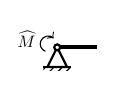
\begin{tikzpicture}[scale=0.25, baseline={(0,-0.1)}]
    \useasboundingbox (-1.5,-1.5) rectangle (2.5,1);
    \draw[line width=1.5pt] (0,0) -- (2,0);
    %\draw[decorate, decoration={snake, amplitude=0.4, segment length=4}] (2,-0.1) -- (2,0.1);
    \draw[thick] (0,0) -- (-0.5, -1) -- (0.5, -1) -- cycle;
    \draw[thick, fill=white] (0,0) circle (0.15);
    \fill[pattern=north east lines] (-0.7,-1.2) rectangle (0.7,-1);
    \draw (-0.7,-1) -- (0.7,-1);
    \draw[->] (-0.6, -0.2) arc (250:45:0.4) node[left, pos=0.5, scale=0.6] {$\widehat{M}$};
\end{tikzpicture}
& 0 & & $\widehat{M}$ & \\

Slider/Guided &
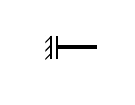
\begin{tikzpicture}[scale=0.25, baseline={(0,-0.1)}]
    \useasboundingbox (-1.5,-1.5) rectangle (2.5,1);
    \draw[line width=1.5pt] (0,0) -- (2,0); 
    %\draw[decorate, decoration={snake, amplitude=0.4, segment length=4}] (2,-0.1) -- (2,0.1);
    \draw[thick] (0,-0.6) -- (0,0.6); 
    \draw[thick] (-0.3,-0.6) -- (-0.3,0.6); 
    \fill[pattern=north east lines] (-0.6,-0.6) rectangle (-0.3,0.6);
\end{tikzpicture}
& & 0 & & 0 \\

Mom. + Force &
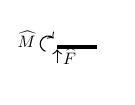
\begin{tikzpicture}[scale=0.25, baseline={(0,-0.1)}]
    \useasboundingbox (-1.5,-1.5) rectangle (2.5,1);
    \draw[line width=1.5pt] (0,0) -- (2,0);
    %\draw[decorate, decoration={snake, amplitude=0.4, segment length=4}] (2,-0.1) -- (2,0.1);
    \draw[->] (-0.6, -0.2) arc (250:45:0.4) node[left, pos=0.5, scale=0.6] {$\widehat{M}$};
    \draw[->] (0,-0.8) -- (0,-0.1) node[right, pos=0.5, scale=0.6] {$\widehat{F}$};
\end{tikzpicture}
& & & $\widehat{M}$ & $\widehat{F}$ \\
\bottomrule
\end{tabular}
\end{center}
Write down equations for each BC using the expressions from Step 3 involving $C_1, C_2, C_3, C_4$.

\step{5} \textbf{Solve Theory Constants}
Solve the system of linear equations for $C_1, C_2, C_3, C_4$.
Substitute back to get final $w(x), \beta(x), M(x), V(x)$.

\step{6} \textbf{Discontinuities (Multi-Region)}
If load $p_z$ changes or supports exist in span (e.g., continuous beam):
\begin{enumerate}
    \item Split into regions (0 to $L_1$, $L_1$ to $L_2$).
    \item Apply Steps 2-3 for EACH region (constants $C_1^I...C_4^I$, $C_1^{II}...C_4^{II}$).
    \item Apply \textbf{Matching Conditions} at $x=L$: 
    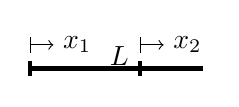
\begin{tikzpicture}{scale=0.25, baseline={(0,0.1)}}
        \draw[line width=1.5pt] (0,0) -- (2.2,0);
        \draw[|->] (0,0.3) -- (0.3,0.3) node[right] {$x_1$};
        \draw[|->] (1.4,0.3) -- (1.7,0.3) node[right] {$x_2$};
        \draw[-, line width=1.5pt] (0,0.1) -- (0,-0.1);
        \draw[-, line width=1.5pt] (1.4,0.1) -- (1.4,-0.1) node[above left] {$L$};
    \end{tikzpicture}
    \begin{itemize}
        \item Continuity: $w_I(L) = w_{II}(0)$, $\beta_I(L) = \beta_{II}(0)$.
        \item Equilibrium: $M_I(L) = M_{II}(0)$, $V_I(L) = V_{II}(0)$ (add point load/moment if present as jumps by 'Auflager').
    \end{itemize}
\end{enumerate}
$w^{shear} = $ all terms with $\frac{1}{GA_V}$; $w^{bending}=$ all terms with $\frac{1}{EI}$.

\section{2. Plates}
\subsection{Theory Overview}
2D structures ($t \ll L_x, L_y$).
\begin{itemize}[leftmargin=*]
    \item \textbf{Reissner-Mindlin (RM)}: Shear deformable. Indep. rotations $\varphi_x, \varphi_y$. Analog to Timoshenko.
    \item \textbf{Kirchhoff-Love (KL)}: Shear rigid. $\varphi \approx \nabla w$. Analog to Euler-Bernoulli.
\end{itemize}

\subsection{Problem Solving Strategy: Plates}

\step{1} \textbf{Classify Problem Type}
\begin{itemize}
    \item Rectangular Plate? $\rightarrow$ Cartesian $(x,y)$.
    \item Circular Plate? $\rightarrow$ Polar $(r, \theta)$.
    \item Axisymmetric? $\rightarrow$ $w=w(r)$ only.
\end{itemize}

\step{2} \textbf{Governing Equations}
\textbf{Case A: Kirchhoff (Thin Plate)}
Solve Biharmonic Equation:
\[ \Delta\Delta w = \frac{p}{K}, \quad K = \frac{Et^3}{12(1-\nu^2)} \]
For Axisymmetric Circular Plate:
\[ \frac{1}{r} \frac{d}{dr} \left\{ r \frac{d}{dr} \left[ \frac{1}{r} \frac{d}{dr} \left( r \frac{dw}{dr} \right) \right] \right\} = \frac{p}{K} \]
Integrate 4 times: $w(r) = C_1 + C_2 r^2 + C_3 \ln r + C_4 r^2 \ln r + w_{part}$.

\textbf{Case B: Reissner-Mindlin}
Solve coupled system for $w, \varphi_x, \varphi_y$.
Often reduces to Kirchhoff solution + Shear correction terms.

\step{3} \textbf{Boundary Conditions (BCs)}
\begin{center}
\scriptsize
\renewcommand{\arraystretch}{1.2}
\begin{tabular}{@{}l p{3.5cm} p{4cm}@{}}
\toprule
\textbf{Support} & \textbf{Kirchhoff (KL)} & \textbf{Reissner-Mindlin (RM)} \\
\midrule
Clamped & $w=0, \partial w/\partial n = 0$ & Hard: $w=0, \varphi_n=0, \varphi_s=0$ \\
& & Soft: $w=0, \varphi_n=0, M_{ns}=0$ \\
\addlinespace
Simply Sup. & $w=0, M_n=0$ & Hard: $w=0, M_n=0, \varphi_s=0$ \\
& & Soft: $w=0, M_n=0, M_{ns}=0$ \\
\addlinespace
Free & $M_n=0$ & $M_n=0$ \\
& $V_{eff} = Q_n + \partial_s M_{ns} = 0$ & $Q_n=0, M_{ns}=0$ \\
\bottomrule
\end{tabular}
\end{center}

\step{4} \textbf{Solution Methods (Rectangular)}
\textbf{Navier's Method} (All sides simply supported):
Expand load $p$ and deflection $w$ in Fourier sine series.
\[ w(x,y) = \sum_{m} \sum_{n} w_{mn} \sin(\alpha_m x) \sin(\beta_n y) \]
Substitute into $\Delta\Delta w = p/K$ to find $w_{mn}$.

\textbf{Levy's Method} (Two opposite sides simply supported):
$w(x,y) = \sum Y_m(y) \sin(\alpha_m x)$.
Solve ODE for $Y_m(y)$.

\section{3. Torsion (Saint-Venant)}
\subsection{Theory Overview}
Twisting of bars ($M_T$).
$\vartheta'$: Rate of twist. $I_T$: Torsional constant.
\[ M_T = G I_T \vartheta' \]

\subsection{Problem Solving Strategy: Torsion}

\step{1} \textbf{Identify Cross-Section Type}
\begin{enumerate}
    \item \textbf{Circular}: Exact solution. $I_T = I_p = \frac{\pi r^4}{2}$.
    \item \textbf{Thin-Walled Open} (I-beam, C-channel):
    $I_T \approx \sum \frac{1}{3} b_i t_i^3$.
    Shear stress $\tau_{max} \approx G t \vartheta'$.
    \item \textbf{Thin-Walled Closed} (Box, Tube):
    Use \textbf{Bredt's Formulas}.
\end{enumerate}

\step{2} \textbf{Closed Sections (Bredt's)}
\begin{itemize}
    \item Shear Flow $q$: Constant in the wall.
    \[ q = \frac{M_T}{2 A_m} \]
    ($A_m$: area enclosed by midline).
    \item Shear Stress: $\tau = q/t$.
    \item Torsional Constant:
    \[ I_T = \frac{4 A_m^2}{\oint \frac{ds}{t}} \]
\end{itemize}

\step{3} \textbf{Multi-Cell Closed Sections}
\begin{itemize}
    \item Flows $q_1, q_2...$ in each cell.
    \item Equilibrium: $M_T = 2 \sum A_i q_i$.
    \item Compatibility: Twist $\vartheta'$ must be same for all cells.
    \[ \vartheta' = \frac{1}{2G A_i} \oint_{\text{cell } i} \frac{q}{t} ds \]
    Solve system for $q_i$.
\end{itemize}

\section{4. Trusses}

\subsection{Theory Overview}
Bars carry only axial force. Nodes are hinges.
Governing Eq: $\mathbf{K}\mathbf{u} = \mathbf{f}$.

\subsection{Problem Solving Strategy: Trusses}

\step{Check} \textbf{Static Determinacy:} 
$f(x) = 2k-s-r = 2\text{\#nodes}-\text{\#bars}-\text{\#support reactions}$. 
If $f=0$, statically determinate. Determine forces by nodal equilibrium or (A,B,C). 
If $f>0$, statically indeterminate. Need extra relationship. 
If $f<0$, statically indeterminate. Need stiffness method (C).

(A) If $f=0$ \textbf{Elongation of bar i:} $\Delta l_i = \frac{N_i l_i}{EA}$ 1) Normal force $N_i$ 2) Plugin $\Delta l_i$. 

(B) \textbf{Unit vector: } $e_{0,i}$ of bar $i$ between nodes $A$, $B$. $e_{0,i} = (x_B-x_A, y_B-y_A)^T$

(C) \textbf{Relationship } $\Delta l_i$ and velocity vector $q_i=(u_i, w_i)^T$: 1) $\Delta l_i$ 2) $e_i's$ 3) $\Delta l_i = e_{0,i} (q_{B,i} - q_{A,i}) = \bm{Aq} \rightarrow \bm{q}$.
$\bm{\Delta l}=(\Delta l_1, \Delta l_2, \cdots)^T, \bm{q} = (u_1, w_1, u_2, w_2, \cdots)^T$.

(D) If $f<0$ \textbf{Stiffness Method (Indeterminate)}
\begin{enumerate}
    \item Define Global DOFs (displacements at nodes).
    \item Element Stiffness Matrix (local $\to$ global coords).
    \[ \mathbf{k}^{(e)} = \frac{EA}{L} \begin{bmatrix} c^2 & cs & -c^2 & -cs \\ cs & s^2 & -cs & -s^2 \\ ... \end{bmatrix} \]
    ($c=\cos\alpha, s=\sin\alpha$).
    \item Assemble Global $\mathbf{K}$.
    \item Apply BCs (remove rows/cols for fixed DOFs).
    \item Solve $\mathbf{K}\mathbf{u} = \mathbf{f}$.
    \item Calculate Forces: $S = \frac{EA}{L} (u_{axial}^{diff})$.
\end{enumerate}

\section{5. Shells}
\subsection{Theory Overview}
Curved structures. Comparison to plates:
\begin{itemize}
    \item \textbf{Membrane Action}: Efficient load carrying via in-plane forces ($N_{xx}, N_{yy}, N_{xy}$).
    \item \textbf{Bending Action}: Additional resistance via moments (less efficient).
\end{itemize}

\subsection{7-Parameter Model}
Advanced formulation to avoid Locking.
Detailed kinematics:
\[ \mathbf{u} = \mathbf{v} + \theta^3 \mathbf{w} + (\theta^3)^2 \tilde{\mathbf{w}} \]
Includes thickness stretch to allow 3D constitutive laws without numerical issues (Poisson locking).

\section{6. Variational Principles (FEM Basis)}
Use when exact analytical solution is difficult.

\step{1} \textbf{Principle of Virtual Work}
\[ \delta W_{int} = \delta W_{ext} \]
\[ \int_V \boldsymbol{\sigma} : \delta\boldsymbol{\epsilon} \, dV = \int \mathbf{p} \cdot \delta\mathbf{u} \, dV + ... \]

\step{2} \textbf{Ritz Method (Approximate)}
\begin{enumerate}
    \item Assume ansatz $w(x) \approx \sum c_i \phi_i(x)$.
    \item $\phi_i(x)$ must satisfy Kinematic BCs ($w=0, w'=0$).
    \item Substitute into $\Pi_{total}$ (Potential Energy).
    \item Minimize: $\frac{\partial \Pi}{\partial c_i} = 0$.
    \item Solve for $c_i$.
\end{enumerate}

\end{multicols*}

\end{document}
